
% arara: pdflatex
\documentclass{article}
\usepackage{graphicx} % For including images
\usepackage{adjustbox} % For adjusting image sizes
\usepackage{longtable}
\usepackage{chemformula}
\usepackage[margin=0.1in]{geometry}
\begin{document}
\section*{s66x8}
\begin{table}[h!]
\begin{center}
\begin{tabular}{|c|c|c|c|}
\hline
Functional & Basis Set & MAE & ME \\
\hline
SAPT0 & adz & 0.46 & 0.23 \\SAPT0 & atz & 0.38 & -0.02 \\SAPT2+3(CCD)DMP2 & adz & 0.22 & 0.22 \\SAPT2+3(CCD)DMP2 & atz & 0.00 & 0.00 \\SAPT(DFT) [PBE0] & adz & 0.57 & 0.57 \\SAPT(DFT) [PBE0] & atz & 0.27 & 0.26 \\PBE0-D4 & adz & 3.91 & 3.91 \\PBE0-D4 & atz & 3.91 & 3.91 \\\hline
\end{tabular}
\caption{Error statistics are in kcal/mol versus SAPT2+3(CCD)DMP2 DISP ENERGY atz}
\end{center}
\end{table}
\clearpage
\begin{figure}[ht]
    \centering
    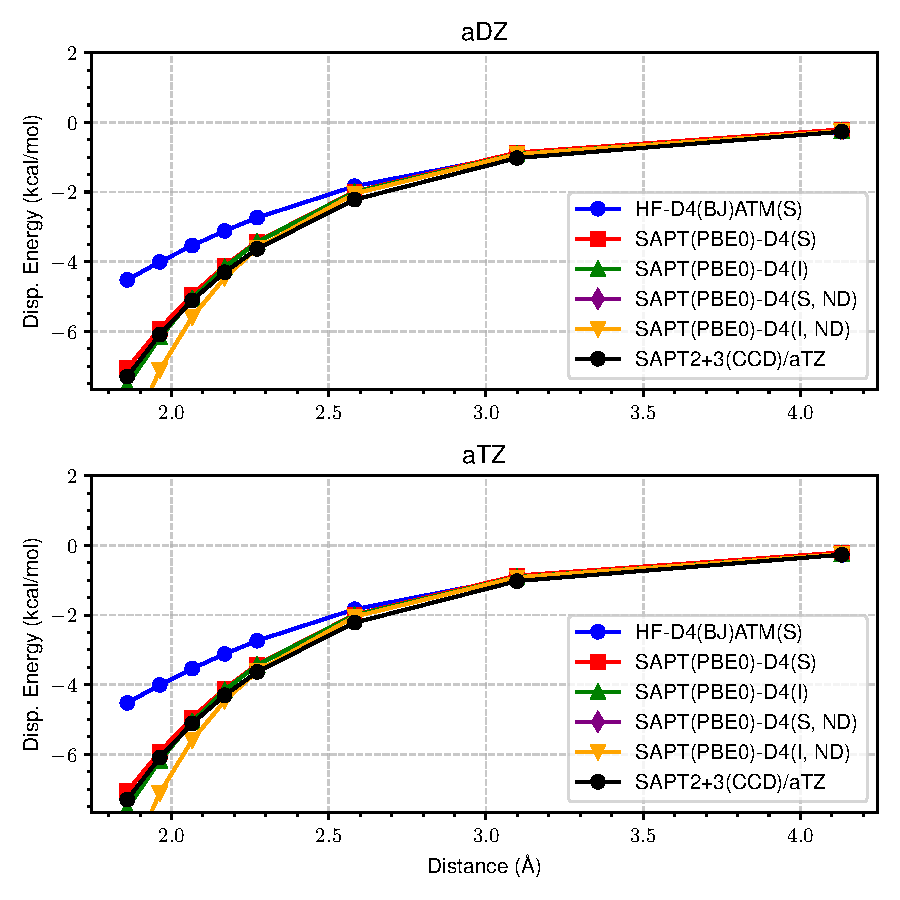
\includegraphics[width=0.7\textwidth]{s66x8/14_Peptide-MeNH2_ddft_super_ddft_curve.pdf}
    \caption{LoS Dispersion Curves for \textbf{s66x8 14\_Peptide-MeNH2}}.
\end{figure}

\clearpage

\begin{figure}[ht]
    \centering
    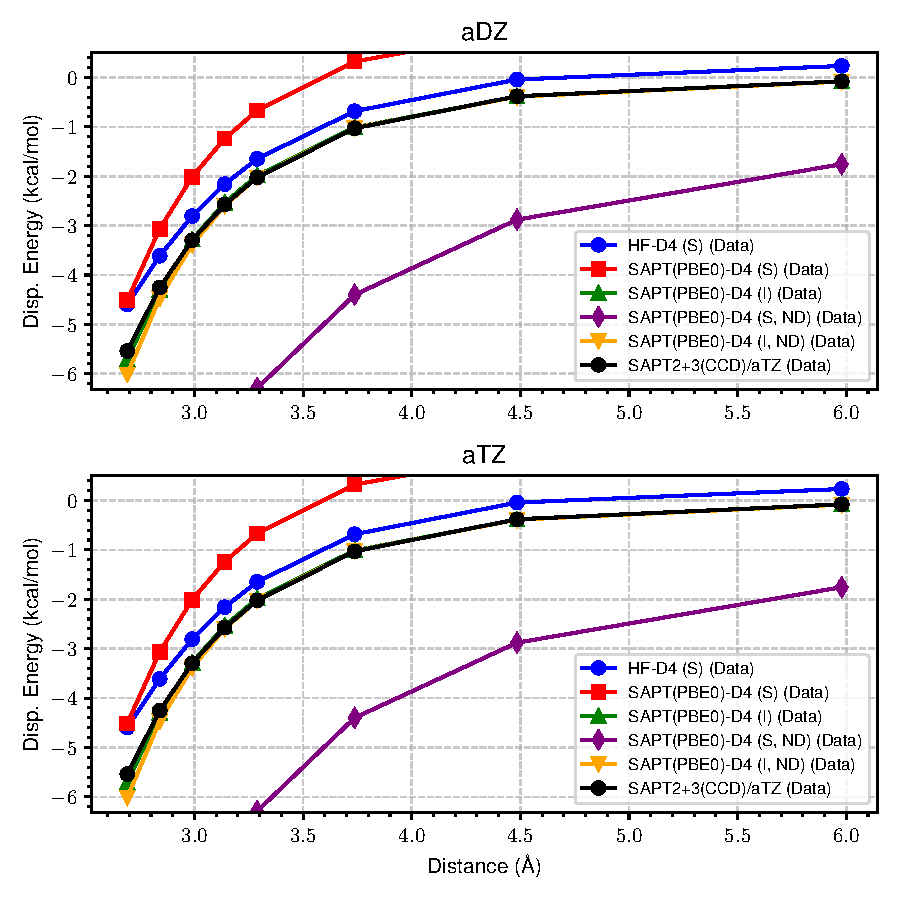
\includegraphics[width=0.7\textwidth]{s66x8/45_Ethyne-Pentane_ddft_super_ddft_curve.pdf}
    \caption{LoS Dispersion Curves for \textbf{s66x8 45\_Ethyne-Pentane}}.
\end{figure}

\clearpage

\begin{figure}[ht]
    \centering
    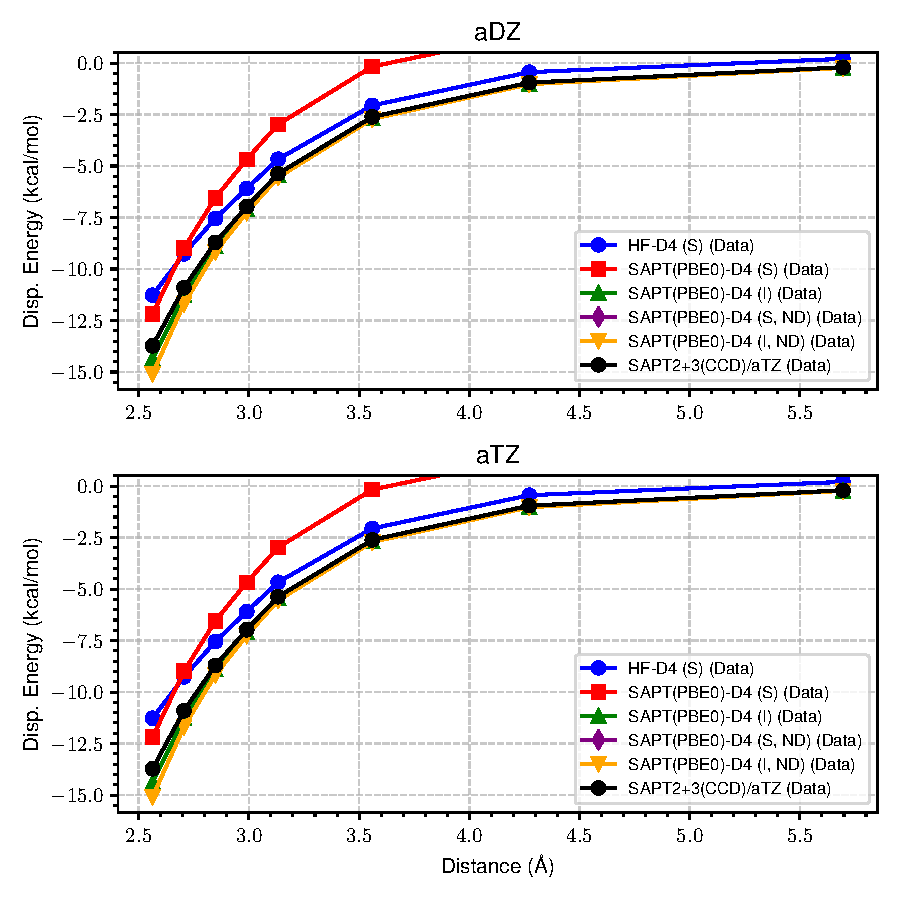
\includegraphics[width=0.7\textwidth]{s66x8/41_Uracil-Pentane_ddft_super_ddft_curve.pdf}
    \caption{LoS Dispersion Curves for \textbf{s66x8 41\_Uracil-Pentane}}.
\end{figure}

\clearpage

\end{document}